\documentclass[aspectratio=169]{beamer}

\usetheme{metropolis}

\usepackage{amsmath}
\usepackage{amssymb}
\usepackage{amsthm}
\usepackage{mathtools}
\usepackage{xcolor}
\usepackage{physics}
\usepackage{bm}
\usepackage{tikz}
\usepackage{pgfplots}
\pgfplotsset{compat=1.18}
\usepackage{svg}
\usepackage{graphicx}
\usepackage{subcaption}
\usepackage{verbatim}

\newcommand{\dimterm}[2]{\alt<1>{#2}{\alt<#1>{#2}{{\color{black!20}#2}}}}

\title{Stokes flow in a lid-driven cavity}
\author{Lukas Lanik}
\date{\today}

\begin{document}

\begin{frame}
  \titlepage
\end{frame}

\begin{frame}{\Large The problem at hand}
  \Large
  Studying the flow of a viscuous fluid in a 2D cavity
\begin{center}
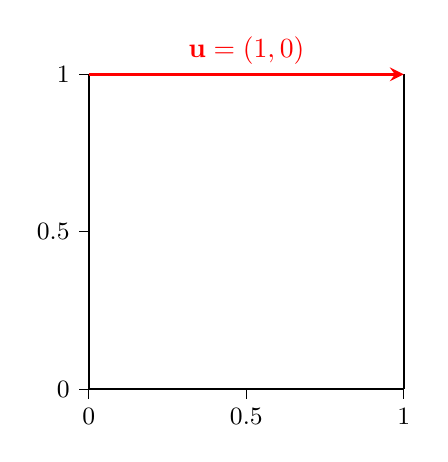
\begin{tikzpicture}[scale=4]
    % Draw grid / ticks
    \draw[help lines, color=gray!30, dashed] (0,0) grid (1,1);
    
    % Axis ticks along the bottom and left edges
    \foreach \x in {0, 0.5, 1}
        \draw (\x,0) -- (\x,-0.03) node[below] {\small\x};
    \foreach \y in {0, 0.5, 1}
        \draw (0,\y) -- (-0.03,\y) node[left] {\small\y};

    % Square outline (bottom, left, and right edges)
    \draw[thick] (0,0) -- (1,0); % bottom
    \draw[thick] (0,0) -- (0,1); % left
    \draw[thick] (1,0) -- (1,1); % right

    % Top edge as a red arrow pointing to the right
    \draw[red, very thick, -stealth] (0,1) -- (1,1);

    % Label the red arrow with u = (1, 0)
    \node[above, red] at (0.5, 1) {$\mathbf{u} = (1, 0)$};
\end{tikzpicture}
\end{center}
\end{frame}

\begin{frame}{\Large Expected resut}
  \begin{figure}[htbp]
    \centering
    \begin{subfigure}[b]{0.45\textwidth}
      \centering
      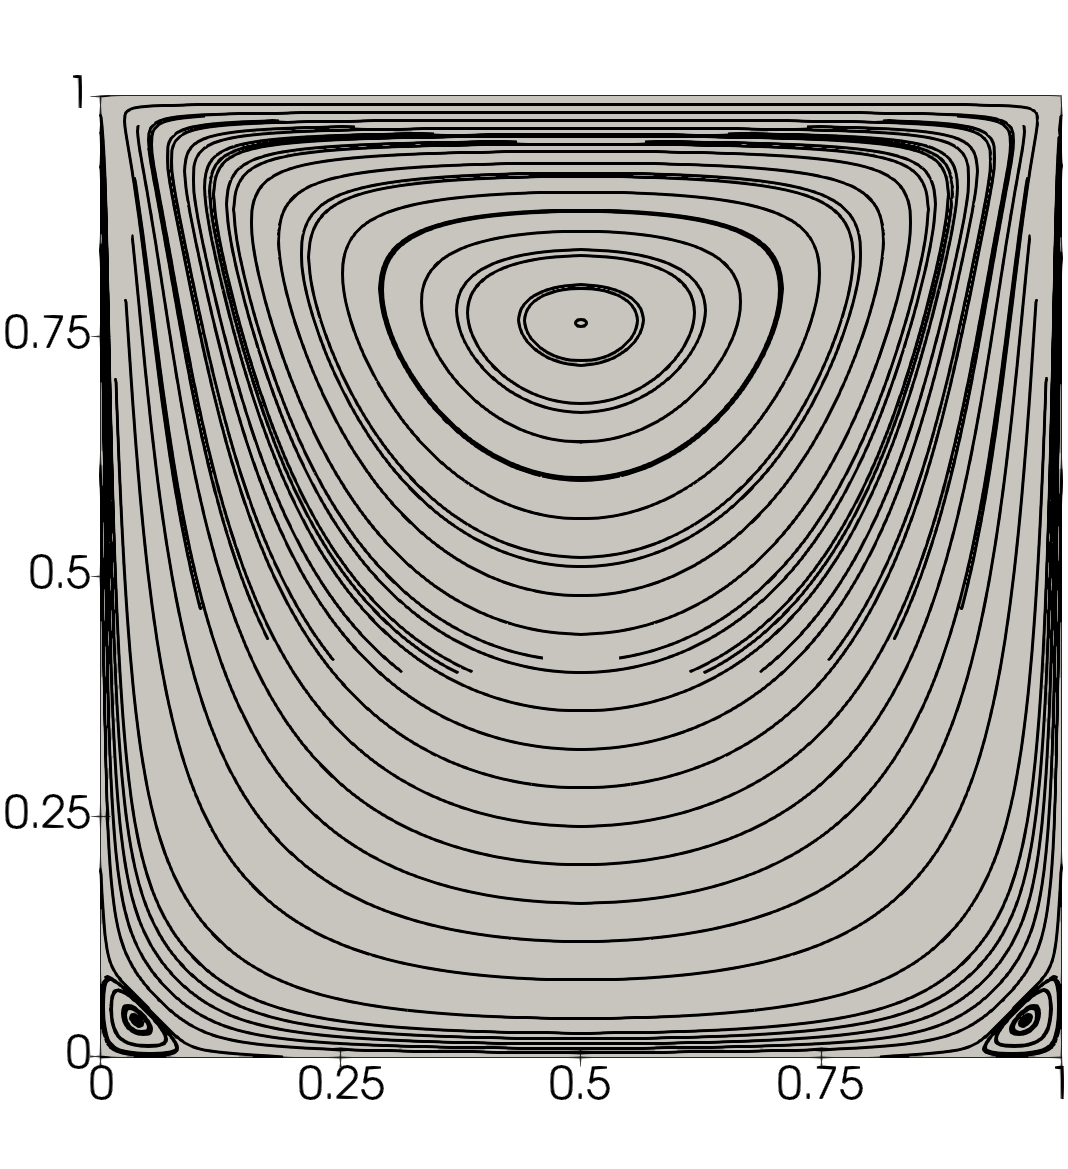
\includegraphics[width=\textwidth]{./images/cavity_P2-P1_128_velocity.png}
      \caption{Velocity streamlines}
      \label{fig:first_image}
    \end{subfigure}
    \begin{subfigure}[b]{0.45\textwidth}
      \centering
      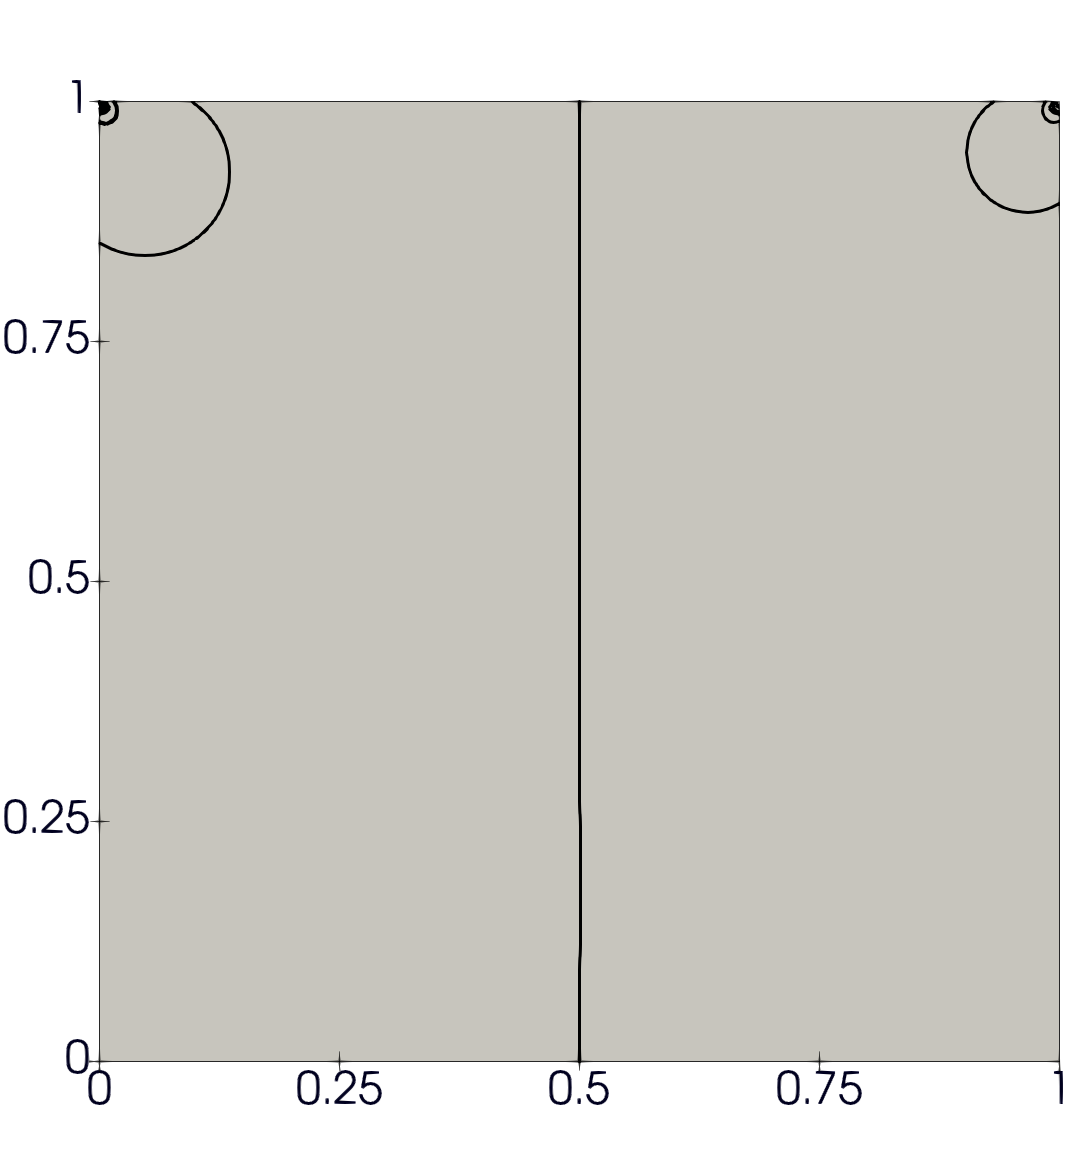
\includegraphics[width=\textwidth]{./images/cavity_P2-P1_128_pressure.png}
      \caption{Pressure isolines}
      \label{fig:second_image}
    \end{subfigure}
  \end{figure}
\end{frame}

\begin{frame}{\Large Navier-Stokes equations}
  \centering
  \Large
  \begin{equation*}
  \begin{cases}
    \frac{\partial \mathbf{u}}{\partial t}
    - \operatorname{div}\left[\nu\left(\nabla \mathbf{u} + \nabla \mathbf{u}^T\right)\right]
    + (\mathbf{u} \cdot \nabla)\mathbf{u}
    + \nabla p
    = \mathbf{f}, & \mathbf{x} \in \Omega, \, t > 0, \\[10pt]
    \operatorname{div} \mathbf{u} = 0, & \mathbf{x} \in \Omega, \, t > 0,
  \end{cases}
  \end{equation*}

  \vspace{0.8cm}

  Complete Incompressible Navier-Stokes System
\end{frame}

\begin{comment}
\begin{frame}{\Large No forcing term and constant viscosity}
  \Large
  \onslide<1->{\begin{equation*}
    \operatorname{div}\left[\nu\left(\nabla \mathbf{u} + \nabla \mathbf{u}^T\right)\right] 
    = \nu \left(\Delta \mathbf{u} + \nabla \operatorname{div} \mathbf{u} \right) 
    = \nu \Delta \mathbf{u}
  \end{equation*}
  }

  \onslide<2->{\begin{equation*}
    \begin{cases}
      \frac{\partial \mathbf{u}}{\partial t} 
      - \nu \Delta \mathbf{u} 
      + (\mathbf{u} \cdot \nabla)\mathbf{u} 
      + \nabla p = 0, & \mathbf{x} \in \Omega, \, t > 0, \\[5pt]
      \operatorname{div} \mathbf{u} = 0, & \mathbf{x} \in \Omega, \, t > 0,
    \end{cases}
  \end{equation*} 
  }
\end{frame}
\end{comment}

\begin{frame}{\Large Non-dimensionalisation}
  \Large
  Units for the terms in the equation
  \begin{equation*}
    [\nu] = \frac{L^2}{T}, \quad [u] = \frac{L}{T}, \quad [p] = \frac{L^2}{T^2} \quad (\text{kinematic pressure})
  \end{equation*}
  \pause
  Choose reference quantities
  \begin{itemize}
    \item characteristic length $L$
    \item characterisitc velocity $U$
  \end{itemize}
  \pause
  Defining dimensionless variables 
  \begin{equation*}
    x = L x^*, \quad t = \frac{L}{U} t^*, \quad u = U u^*, \quad p = U^2 p^*
  \end{equation*}
\end{frame}

\begin{frame}{\Large Non-dimensionalisation}
  \Large
  Each term is transformed
  \begin{align*}
    \frac{\partial \mathbf{u}}{\partial t} &= \frac{U^2}{L} \frac{\partial \mathbf{u}^*}{\partial t} \\
    -\nu \Delta \mathbf{u} &= -\frac{\nu U}{L^2}\Delta^* \mathbf{u}^* \\
    (\mathbf{u} \cdot \nabla) \mathbf{u} &= \frac{U^2}{L} (\mathbf{u}^* \cdot \nabla^*) \mathbf{u}^* \\
    \nabla p &= \frac{U^2}{L} \nabla^* p^*
  \end{align*}
\end{frame}

\begin{frame}{\Large Non-dimensionalisation}
  \Large
  Plugging in the transformed terms and dividing by $\frac{U^2}{L}$ gives
  \begin{equation*}
      \frac{\partial \mathbf{u}^*}{\partial t^*} 
      - \frac{\nu}{UL} \Delta^* \mathbf{u}^* 
      + (\mathbf{u}^* \cdot \nabla^*)\mathbf{u}^* 
      + \nabla^* p^* = 0
  \end{equation*}
  Define
  \begin{equation*}
    \mathrm{Re} = \frac{UL}{\nu}
  \end{equation*}
  hence
  \begin{equation*}
      \frac{\partial \mathbf{u}^*}{\partial t^*} 
      - \frac{1}{\mathrm{Re}} \Delta^* \mathbf{u}^* 
      + (\mathbf{u}^* \cdot \nabla^*)\mathbf{u}^* 
      + \nabla^* p^* = 0
  \end{equation*}
\end{frame}


\begin{frame}{\Large Stokes regime Re $\rightarrow$ 0}
  \Large
  As the fluid gets more viscuous (Re $\rightarrow$ 0) turbulence disappears
  thus time derivative can be neglected.
  \begin{equation*}
    \begin{cases}
      -\Delta \mathbf{u} 
      + \nabla p = 0, & \mathbf{x} \in \Omega \\[5pt]
      \operatorname{div} \mathbf{u} = 0, & \mathbf{x} \in \Omega
    \end{cases}
  \end{equation*}
  \begin{align*}
    \mathbf{u} &= \mathbf{0}, \qquad\mathbf{x} \in \partial\Omega \setminus \varGamma, \\[5pt]
    \mathbf{u} &= (1,0)^T, \qquad \mathbf{x} \in \varGamma,
  \end{align*}
  \centering
  where $\varGamma = \{\mathbf{x} = (x_1, x_2)^T \in \partial \Omega: x_2 = 1\}$
\end{frame}

\begin{comment}
\begin{frame}{\Large Weak formulation of Stokes problem}
\Large
Let $v \in V$ and $q \in Q$
  \begin{equation*}
    -\int_{\Omega} \Delta \mathbf{u} \cdot \mathbf{v} \, d\Omega 
    + \int_{\Omega} \nabla p \cdot \mathbf{v} \, d\Omega 
    = 0
  \end{equation*}

  \begin{equation*}
    \int_{\Omega} (\operatorname{div} \mathbf{u}) \, q \, d\Omega = 0
  \end{equation*}
\end{frame}

\begin{frame}{\Large Reduction of order}
\Large
  \begin{equation*}
    -\int_{\Omega} \Delta \mathbf{u} \cdot \mathbf{v} \, d\Omega 
    = \int_{\Omega} \nabla \mathbf{u} \cdot \nabla \mathbf{v} \, d\Omega 
    - \int_{\partial \Omega} \frac{\partial \mathbf{u}}{\partial \mathbf{n}} \cdot \mathbf{v} \, d\gamma 
  \end{equation*}

  \begin{equation*}
    \int_{\Omega} \nabla p \cdot \mathbf{v} \, d\Omega 
    = -\int_{\Omega} p \operatorname{div} \mathbf{v} \, d\Omega 
    + \int_{\partial \Omega} p \mathbf{v} \cdot \mathbf{n} \, d\gamma 
  \end{equation*}
\end{frame}
\end{comment}

\begin{frame}{\Large Weak formulation of the Stokes problem}
  \Large
  Find $(\mathbf{u}, p) \in V \times Q$ such that
  \begin{equation*}
    \begin{cases}
      a(\mathbf{u}, \mathbf{v}) + b(\mathbf{v}, p) = 0, & \forall \mathbf{v} \in V \\
      b(\mathbf{u}, q) = 0, & \forall q \in Q
    \end{cases}
  \end{equation*}
  where
  \begin{equation*}
    a(\mathbf{u}, \mathbf{v})
    = \int_{\Omega} \nabla \mathbf{u} \cdot \nabla \mathbf{v} \, d\Omega 
  \end{equation*}
  \begin{equation*}
    b(\mathbf{u}, q)
    = -\int_{\Omega} q\operatorname{div} \mathbf{u} \, d\Omega
  \end{equation*}
\end{frame}

\begin{frame}{\Large Appropriate spaces for V and Q}
  \Large
  Let $\mathbf{v} \in V$ and $q \in Q$
  \begin{equation*}
    V = \{ \mathbf{v} \in \left[ \mathrm{H}^1 (\Omega) \right]^2 : \mathbf{v} \vert_{\varGamma_D} = 0 \}
  \end{equation*}
  \begin{equation*}
    Q = \{q \in \mathrm{L}^2 (\Omega) : \int_{\Omega} q \, d\Omega = 0 \}
  \end{equation*}
  \begin{equation*}
    \int_{\Omega} \nabla \mathbf{u} \cdot \nabla \mathbf{v} \, d\Omega 
    -\int_{\Omega} p \operatorname{div} \mathbf{v} \, d\Omega 
    = 0
  \end{equation*}
  \begin{equation*}
    \int_{\Omega} (\operatorname{div} \mathbf{u}) \, q \, d\Omega = 0
  \end{equation*}
\end{frame}

\begin{frame}{\Large Galerkin approximation}
  \Large
  Let $V_h \subset V$, $Q_h \subset Q$ be finite dimensional subspaces. Find
  $u_h = \sum_{i=0}^{N_h} u_i \varphi_i$,
  $p_h = \sum_{k=0}^{M_h} p_k \phi_k$.

  The Stokes problem becomes
  \begin{equation*}
    \begin{cases}
      \mathsf{A}\mathbf{U} + \mathsf{B}^T \mathbf{P} = 0 \\
      \mathsf{B} \mathbf{U} = 0
    \end{cases}
  \end{equation*}
  
  \begin{equation*}
    \mathsf{A} = [a_{ij}] = [a(\varphi_j, \varphi_i)], \quad \mathsf{B} = [b_{km}] = [b(\varphi_m, \phi_k)] 
  \end{equation*}
\end{frame}

\begin{frame}{\Large The inf-sup condition}
  \Large
  There exists $\beta_h > 0$ such that
  \begin{equation*}
    \forall q_h \in Q_h \,\, \exists v_h \in V_h, \, v_h \neq 0 \,:\, b(v_h, q_h) \geq \beta_h \Vert v_h \Vert_V \Vert q_h \Vert_Q
  \end{equation*}
\end{frame}

\begin{comment}
\begin{frame}{\Large Algebraic system}
  \Large
  \begin{equation*}
    \mathsf{S} =
    \begin{bmatrix}
      \mathsf{A} & \mathsf{B}^T \\
      \mathsf{B} & \mathsf{0}
    \end{bmatrix}
  \end{equation*}

  \begin{equation*}
    \mathbf{U} = -\mathsf{A}^{-1} \mathsf{B}^T \mathbf{P}
  \end{equation*}
  \begin{equation*}
    \mathsf{R} \mathbf{P} = 0, \quad \text{where} \quad \mathsf{R} = \mathsf{B} \mathsf{A}^{-1} \mathsf{B}^T
  \end{equation*}
  The system admits a unique solution for $\mathbf{P}$ iff $\operatorname{ker}\mathsf{B}^T = \{\mathbf{1}\}$
\end{frame}
\end{comment}

\begin{frame}{\Large Unstable P1-P1 elements}
  \Large
  $V = \mathbb{P}_1$, $Q = \mathbb{P}_1$ - continuous, piecewise polynomial functions

  \vspace{15pt}

  \centering 
  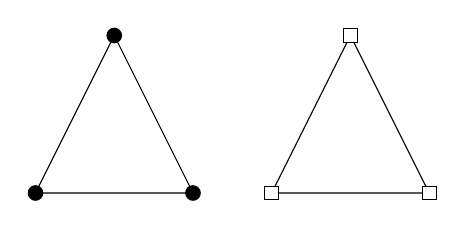
\begin{tikzpicture}[
  % Define styles for the nodes
  dot/.style={circle, fill=black, inner sep=2pt},
  square/.style={rectangle, draw=black, fill=white, inner sep=2.5pt}
  ]

  % --- Left Triangle (Solid Dots) ---
  % Coordinates: Bottom-Left (0,0), Bottom-Right (2,0), Top (1,2)
  \draw (0,0) -- (2,0) -- (1,2) -- cycle;

  \node[dot] at (0,0) {};
  \node[dot] at (2,0) {};
  \node[dot] at (1,2) {};

  % --- Right Triangle (Hollow Squares) ---
  % Offset by x=3 to place it side-by-side
  \draw (3,0) -- (5,0) -- (4,2) -- cycle;

  \node[square] at (3,0) {};
  \node[square] at (5,0) {};
  \node[square] at (4,2) {};
  \end{tikzpicture}

  $\bullet$ represents DOFs for velocity and $\square$ represents DOFs for pressure
\end{frame}

\begin{frame}{\Large Unstable P1-P1 elements}
  \begin{figure}[htbp]
    \centering
    \begin{subfigure}[b]{0.45\textwidth}
      \centering
      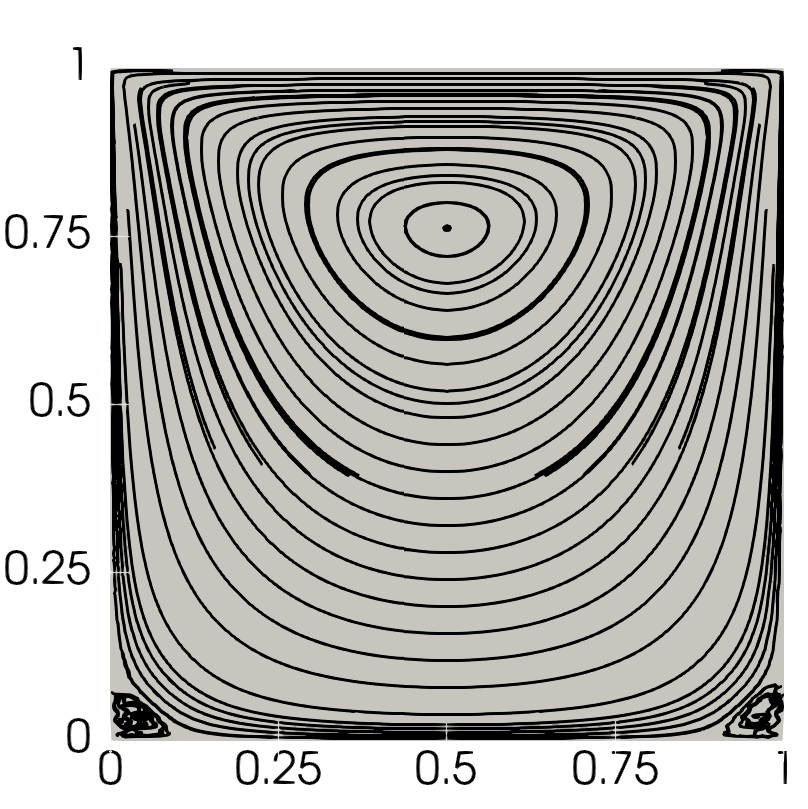
\includegraphics[width=\textwidth]{./images/cavity_P1-P1_128_velocity.png}
      \caption{Velocity streamlines}
      \label{fig:first_image}
    \end{subfigure}
    \begin{subfigure}[b]{0.45\textwidth}
      \centering
      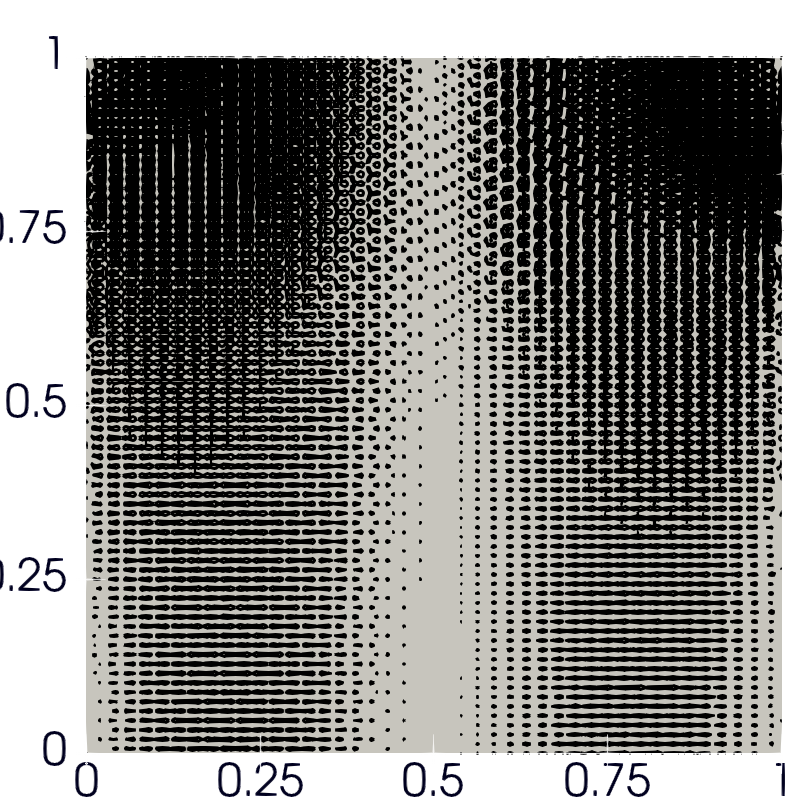
\includegraphics[width=\textwidth]{./images/cavity_P1-P1_128_pressure.png}
      \caption{Pressure isolines}
      \label{fig:second_image}
    \end{subfigure}
  \end{figure}
\end{frame}

\begin{frame}{\Large Constructed pressure modes for P1-P1}
  Assume that $(\mathbf{u_h}, p_h)$ is a solution of the Stokes problem,
  and $(\mathbf{u_h}, q_h^*)$ is as follows:
\begin{center}
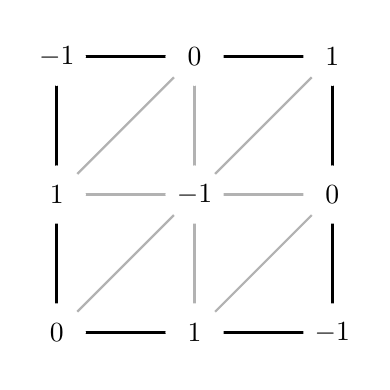
\begin{tikzpicture}[scale=3.5]
    % Coordinates of the grid points for a refined triangulation
    % Vertices: (0,0), (0.5,0), (1,0), (0,0.5), (0.5,0.5), (1,0.5), (0,1), (0.5,1), (1,1)
    
    % Draw the triangulation lines
    \draw[thick, gray!60] (0,0) -- (0.5,0) -- (1,0);
    \draw[thick, gray!60] (0,0.5) -- (0.5,0.5) -- (1,0.5);
    \draw[thick, gray!60] (0,1) -- (0.5,1) -- (1,1);
    
    \draw[thick, gray!60] (0,0) -- (0,0.5) -- (0,1);
    \draw[thick, gray!60] (0.5,0) -- (0.5,0.5) -- (0.5,1);
    \draw[thick, gray!60] (1,0) -- (1,0.5) -- (1,1);

    % Diagonals making up the triangulation
    \draw[thick, gray!60] (0,0) -- (0.5,0.5);
    \draw[thick, gray!60] (0.5,0.5) -- (1,1);
    \draw[thick, gray!60] (0,0.5) -- (0.5,1);
    \draw[thick, gray!60] (0.5,0) -- (1,0.5);

    % Outer square boundary with a stronger stroke
    \draw[very thick] (0,0) rectangle (1,1);

    % Render nodes with background fill to cover grid lines nicely
    \fill[white] (0,0) circle (3pt); \node at (0,0) {$0$};
    \fill[white] (0.5,0) circle (3pt); \node at (0.5,0) {$1$};
    \fill[white] (1,0) circle (3pt); \node at (1,0) {$-1$};
    
    \fill[white] (0,0.5) circle (3pt); \node at (0,0.5) {$1$};
    \fill[white] (0.5,0.5) circle (3pt); \node at (0.5,0.5) {$-1$};
    \fill[white] (1,0.5) circle (3pt); \node at (1,0.5) {$0$};
    
    \fill[white] (0,1) circle (3pt); \node at (0,1) {$-1$};
    \fill[white] (0.5,1) circle (3pt); \node at (0.5,1) {$0$};
    \fill[white] (1,1) circle (3pt); \node at (1,1) {$1$};
\end{tikzpicture}
\end{center}
Then $(\mathbf{u_h}, p_h + q_h^*)$ is a solution with a spurious pressure mode.
\end{frame}

\begin{frame}{\Large Stable P2-P1 elements}
  \Large
  $V = \mathbb{P}_2$, $Q = \mathbb{P}_1$ - any $\mathbb{P}_k, \mathbb{P}_{k-1}$ for $k \geq 2$ is stable

  \vspace{15pt}

  \centering 
  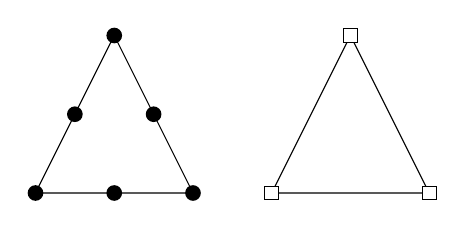
\begin{tikzpicture}[
  % Define styles for the nodes
  dot/.style={circle, fill=black, inner sep=2pt},
  square/.style={rectangle, draw=black, fill=white, inner sep=2.5pt}
  ]

  % --- Left Triangle (Solid Dots) ---
  % Coordinates: Bottom-Left (0,0), Bottom-Right (2,0), Top (1,2)
  \draw (0,0) -- (2,0) -- (1,2) -- cycle;

  \node[dot] at (0,0) {};
  \node[dot] at (1, 0) {};
  \node[dot] at (0.5, 1) {};
  \node[dot] at (1.5, 1) {};
  \node[dot] at (2,0) {};
  \node[dot] at (1,2) {};

  % --- Right Triangle (Hollow Squares) ---
  % Offset by x=3 to place it side-by-side
  \draw (3,0) -- (5,0) -- (4,2) -- cycle;

  \node[square] at (3,0) {};
  \node[square] at (5,0) {};
  \node[square] at (4,2) {};
  \end{tikzpicture}

  $\bullet$ represents DOFs for velocity and $\square$ represents DOFs for pressure 
  
  \normalsize
  Proof of stability for $\mathbb{P}_k, \mathbb{P}_{k-1}$ is given in
  Brezzi \& Fortin, Mixed and Hybrid Finite Element Methods, Springer, 1991
\end{frame}

\begin{frame}{\Large Stable P2-P1 elements}
  \begin{figure}[htbp]
    \centering
    \begin{subfigure}[b]{0.45\textwidth}
      \centering
      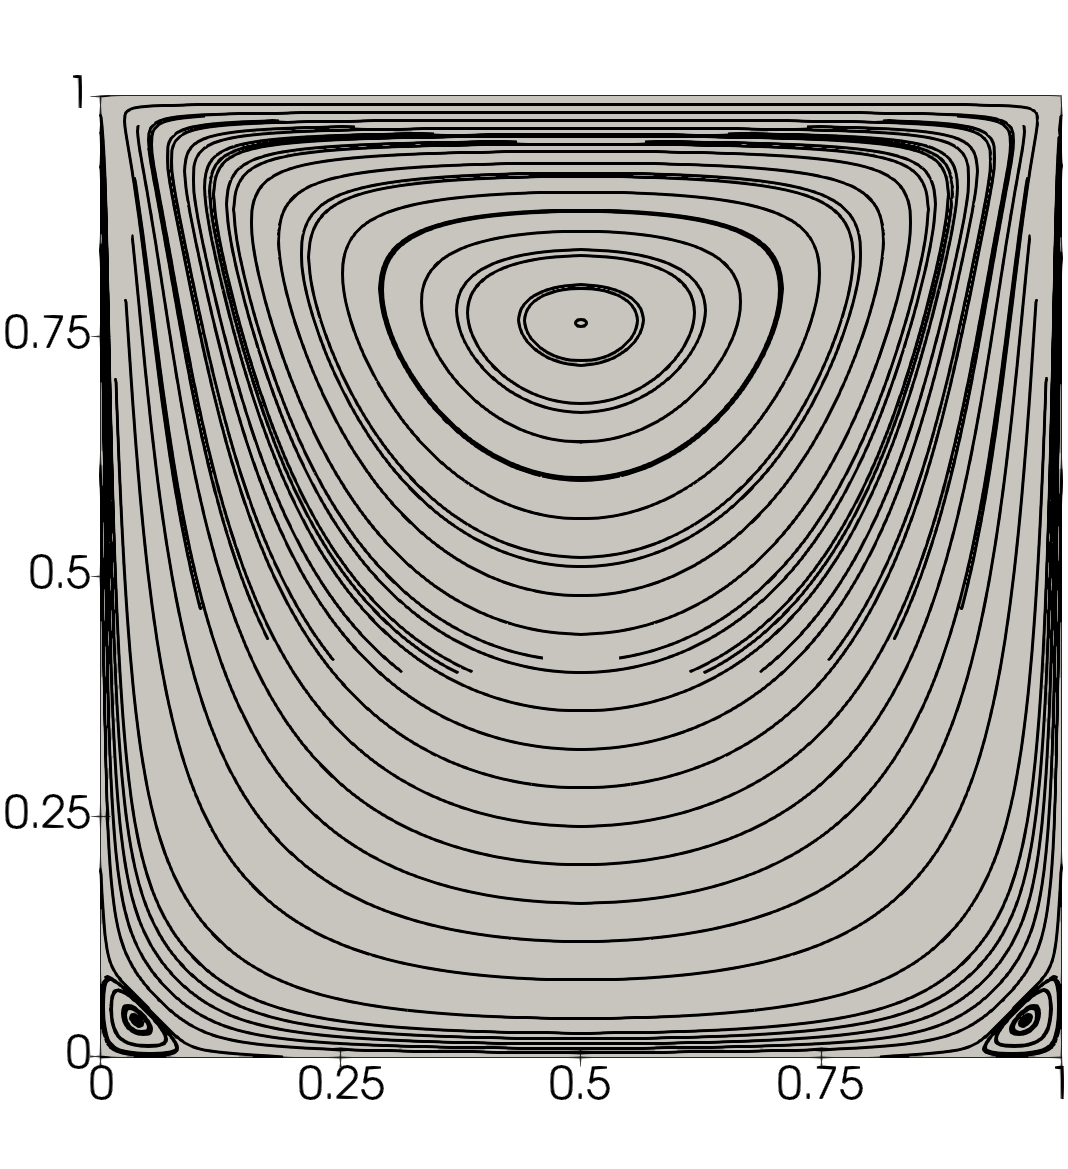
\includegraphics[width=\textwidth]{./images/cavity_P2-P1_128_velocity.png}
      \caption{Velocity streamlines}
      \label{fig:first_image}
    \end{subfigure}
    \begin{subfigure}[b]{0.45\textwidth}
      \centering
      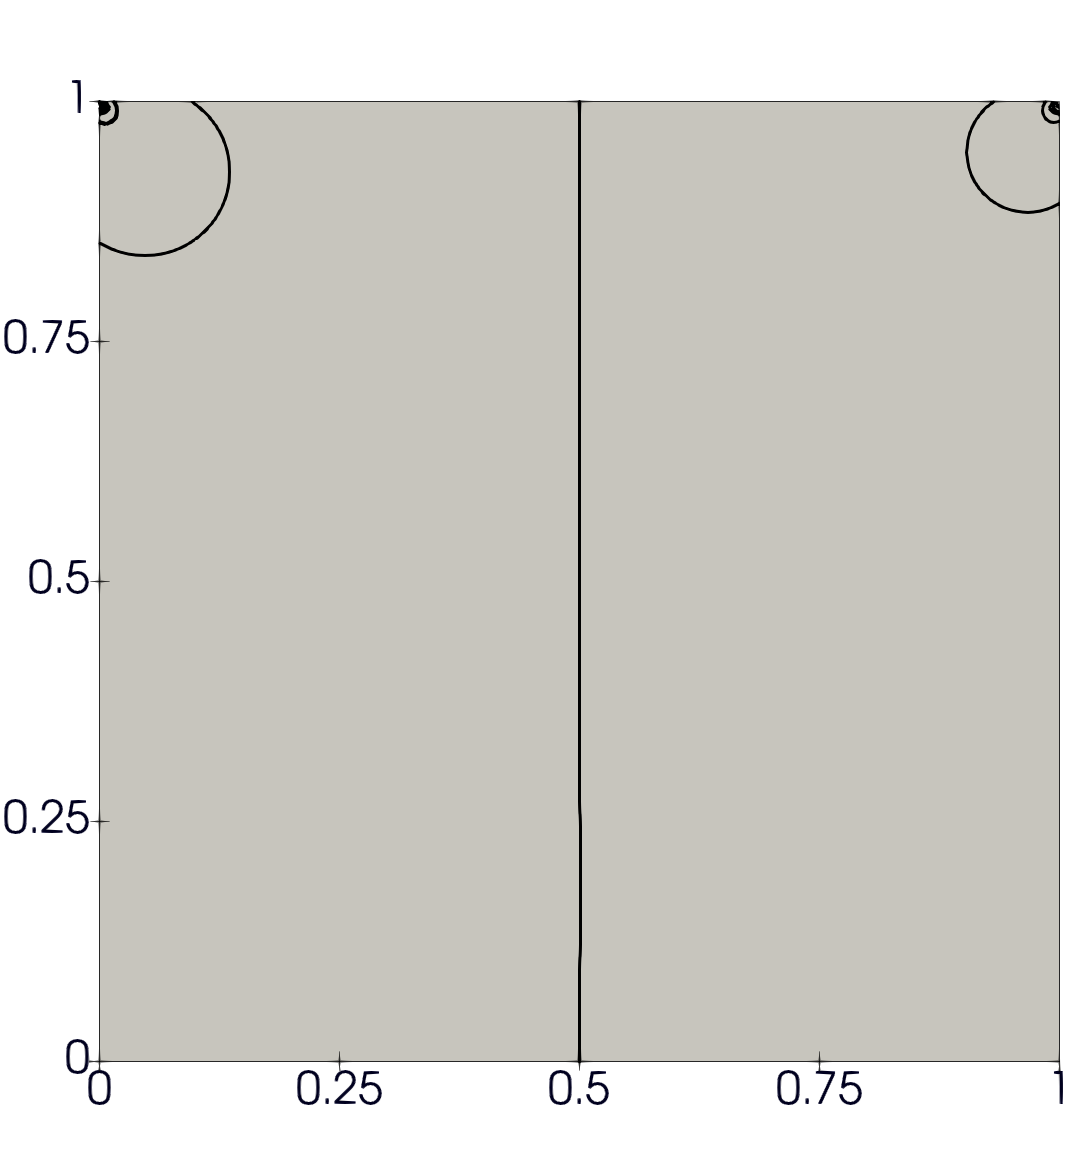
\includegraphics[width=\textwidth]{./images/cavity_P2-P1_128_pressure.png}
      \caption{Pressure isolines}
      \label{fig:second_image}
    \end{subfigure}
  \end{figure}
\end{frame}

\begin{frame}{\Large P1-P1 stabilisation}
  \Large
  Enrich $\mathbb{P}_1$ space with cubic bubble functions. V = $\mathbb{P}_1 \oplus B$ where
  \begin{equation*}
    B = \{p \in \mathbb{P}_3 \, : \, p=0 \quad \text{on the boundary} \}
  \end{equation*}


  \centering 
  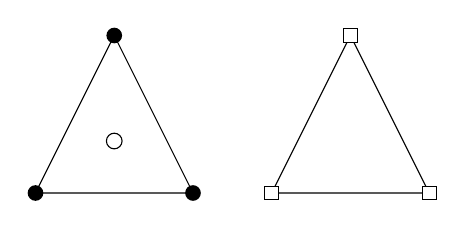
\begin{tikzpicture}[
  % Define styles for the nodes
  dot/.style={circle, fill=black, inner sep=2pt},
  open_circle/.style={circle, draw=black, fill=white, inner sep=2pt},
  square/.style={rectangle, draw=black, fill=white, inner sep=2.5pt}
  ]

  % --- Left Triangle (Solid Dots) ---
  % Coordinates: Bottom-Left (0,0), Bottom-Right (2,0), Top (1,2)
  \draw (0,0) -- (2,0) -- (1,2) -- cycle;

  \node[dot] at (0,0) {};
  \node[dot] at (2,0) {};
  \node[dot] at (1,2) {};
  %
  % Mid-edge nodes (e.g., for P2 velocity) - added three open circles
  \node[open_circle] at (1,0.66) {};   % Mid bottom edge

  % --- Right Triangle (Hollow Squares) ---
  % Offset by x=3 to place it side-by-side
  \draw (3,0) -- (5,0) -- (4,2) -- cycle;

  \node[square] at (3,0) {};
  \node[square] at (5,0) {};
  \node[square] at (4,2) {};
  \end{tikzpicture}

  $\bullet$ velocity DOFs, $\circ$ bubble function DOFs, $\square$ pressure DOFs
  
  \normalsize
  Stability of the bubble elements is shown in D. N. Arnold, F. Brezzi \& M. Fortin (1984),
  "A stable finite element for the Stokes equations"
\end{frame}

\begin{frame}{\Large P1-P1 stabilisation}
  \begin{figure}[htbp]
    \centering
    \begin{subfigure}[b]{0.45\textwidth}
      \centering
      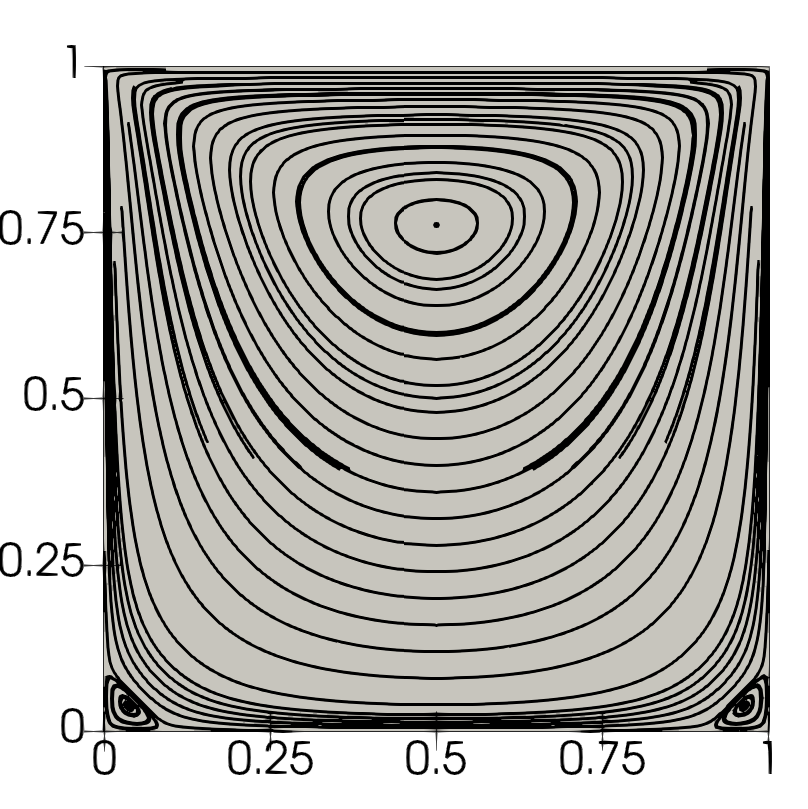
\includegraphics[width=\textwidth]{./images/cavity_P1b-P1_128_velocity.png}
      \caption{Velocity streamlines}
      \label{fig:first_image}
    \end{subfigure}
    \begin{subfigure}[b]{0.45\textwidth}
      \centering
      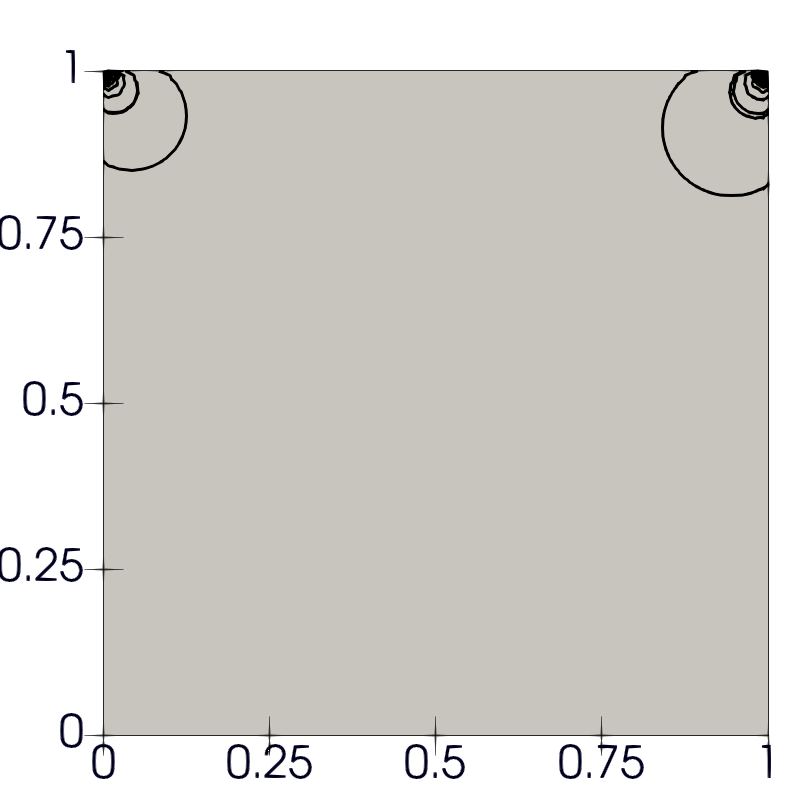
\includegraphics[width=\textwidth]{./images/cavity_P1b-P1_128_pressure.png}
      \caption{Pressure isolines}
      \label{fig:second_image}
    \end{subfigure}
  \end{figure}
\end{frame}

\begin{frame}{\Large Usefullness of AI}
  \Large
  \begin{itemize}
    \item research: valuable suggestions
    \item checking ones reasoning: valuable
    \item niche questions: unsatisfactory
    \item validation data: fabulations
    \item claude vs chatgpt vs u:ai
  \end{itemize}
\end{frame}


\begin{frame}[standout]
  Thank you for your attention!
\end{frame}
\end{document}
